\chapter{Supplementary materials for \autoref{chap:SMME}}
\label{chap:SMMsupp}
\section{Materials and methods}
\subsection{Zebrafish husbandry}
\label{ssec:husbandry}
Zebrafish used in this study were of a wild type AB genetic background. Embryos were derived from pairwise crossings. Larvae were collected upon crossing and held in a dark incubator at 28\textdegree C. At 1dpf, embryos were treated with 100$\mu$l of bleach diluted in 170ml of embryo medium for 3 minutes, rinsed and dechorionated. Embryo medium was changed at 3dpf. After this, all animals were maintained at 28\textdegree C on a 14-hour light/10-hour dark cycle (light intesity of 300 lux) in an automated recirculating aquaculture system (Aquaneering). Animals were reared using standard protocols\cite{Westerfield2000}. Fish were sacrificed by tricaine overdose at the appropriate timepoints indicated in the text. All animal experiments were performed with the approval of the University of Toronto Animal Care Committee in accordance with guidelines from the Canadian Council for Animal Care (CCAC).
 
\subsection{Proliferative RPC Histochemistry}
\subsubsection{Anti-PCNA histochemistry}
In order to assay the number of proliferating cells in zebrafish CMZs, we used anti-PCNA histochemical labelling, as PCNA is, in zebrafish, detectable throughout the cell cycle in proliferating cells. After sacrifice as described above, fish (or their razor-decapitated heads, in the case of fish older than 30dpf) were fixed in 1:9 37\% formaldehyde:95\% ethanol at room temperature (RT) for 30 minutes, followed by overnight incubation in a fridge at 4\textdegree C. Subsequently, the samples were removed from fix and washed 3 times in PBS. They were then cryoprotected by successive 30 minute rinses at RT on a rocker in 5\%, 13\%, 17.5\%, 22\%, and 30\% sucrose in PBS. Samples were allowed to incubate overnight at 4\textdegree C in 30\% sucrose. The next day, samples were removed from the sucrose rinse and infiltrated with 2:1 30\% sucrose:OCT compound (TissueTek) for 30 minutes at RT. Samples were then embedded for cryosectioning and frozen. 14$\mu$m coronal cryosections were cut through the fish's heads and collected on Superfrost slides (Fisherbrand). These were stored in a freezer at -20\textdegree C until staining.

Staining was begun by allowing the slides to dry briefly at RT. Sections were outlined with a PAP pen, then rehydrated in PBS for 30 minutes at RT. Subsequently, sections were blocked in 0.2\% Triton X-100 + 2\% goat serum in PBS for 30 minutes at RT. This was followed by incubation in mouse monoclonal (PC10) anti-PCNA primary antibody (Sigma), diluted 1:1000 in blocking solution, at 4\textdegree C overnight. The next day, primary antibody was removed, and slides were rinsed five times in PDT (PBS + 1\% DMSO + 0.1\% Tween-20). Cy5-conjugated goat-anti-mouse secondary antibody (Jackson Laboratories), diluted 1:100 in blocking solution, was applied to the sections, which were incubated at 37\textdegree C for 2 hours. Secondary antibody was removed, followed by five rinses in PDT as above. Sections were counterstained with Hoechst 33258 diluted to 100 $\mu$g/mL in PBS for 15 minutes at RT. Counterstain was then removed, five rinses in PDT were performed as above, followed by a final rinse in PBS. Slides were then mounted in ProLong Gold antifade mounting medium (ThermoFisher Scientific), coverslipped, and sealed with clear nail polish. Slides were kept at 4\textdegree C until imaging.

\subsubsection{Cumulative thymidine analogue labelling for estimation of CMZ RPC cell cycle length}
In order to obtain an estimate of cell cycle length in CMZ RPCs at 3dpf, we used cumulative thymidine analogue labelling following the method of Nowakowski et al.\cite{Nowakowski1989}. 3dpf zebrafish were divided into ten groups of n\=5 animals and held in 10 mM EdU for 0.5, 1.5, 2.5, 3.5, 4.5, 5.5, 7.5, 8.5, 9.5, and 10.5 hours, after which they were sacrificed as described above. Samples were processed as described under ``Anti-PCNA histochemistry", except that goat-anti-mouse Cy2-conjugated secondary antibody (Jackson Laboratories) was used to label anti-PCNA, after which the Alexa Fluor 647-conjugated azide from a Click-iT kit (ThermoFisher Scientific) was added to the sections for 30 minutes at room temperature to label EdU-bearing nuclei. This was followed by five PDT rinses as described above, and resumption of the protocol with counterstaining, mounting, etc. The raw data is available in \path{\empirical_data\cumulative_edu.xlsx}

\subsubsection{Whole retina thymidine analogue labelling of post-embryonic CMZ contributions}
We used thymidine analogue labelling as an indelible marker of CMZ contributions to the retina in Fig \ref{RingFig}. Because thymidine analogues are incorporated into DNA during S-phase, postmitotic progeny of proliferating RPCs which take up the label may be detected at any point after this treatment. Dosing zebrafish with a thymidine analogue for a limited period of time ensures that the label is diluted to undetectable levels in cells which continue to proliferate. Repetitive dosing thus gives rise to labelled cohorts which represent a limited set of generations of cells which become postmitotic after the dose is provided. n=3 fish were held in 10mM BrdU (Sigma) diluted in facility water for 8 hours at 30, 60, 90, 120, and 150 days post fertilisation. 10 days after the last BrdU incubation, the fish were sacrificed as described above. One representative whole retina dissection is presented.

\subsection{Confocal microscopy and image analysis}
All histochemically processed samples (coronal sections of retinas and whole retinas) were imaged on a Leica TCS SP5 II laser confocal imaging microscope, using the Leica LAS AF software for acquisition. For coronal sections, central sections were identified by their position in the ribbon of cryosections. For Fig \ref{WanSim}, the central section was imaged together with the flanking section on either side of it. Confocal data was analysed using Imaris Bitplane software (v. 7.1.0). Cell counting analyses were performed by segmenting the relevant channels using the Surfaces tool to produce counts of PCNA positive (Figs \ref{WanSim}, \nameref{cumulativeSupplement}) or PCNA/EdU double-positive (\nameref{cumulativeSupplement}) nuclei. Lens diameters were measured in the DIC channel using the linear measurement tools, across the widest point of the section of spherical lens.

\subsection{Estimation of CMZ annular population size}
\label{sec:lenspopest}
In order to estimate the total population of the CMZ in zebrafish eyes sampled throughout the first year of life, we counted PCNA-positive cells in the dorsal and ventral CMZ of central and flanking sections of these eyes as described above. We added the dorsal and ventral populations and took the average of the central and flanking section per-section populations to reduce the possibility of sampling error. We treated this as a sample of a torus mapped to the 14$\mu$m sphere segment of lens intersected by the average section. As the surface area of this zone is given by $S = \pi \times d_{lens} \times h_{section}$, and the total surface area of the lens by $A = \pi \times d_{lens}^2$, where $d$ is the diameter of the lens and $h$ the section thickness, we may calculate an estimate of the total population by $pop_{total} = \frac{pop_{section}}{S} * A$. We therefore obtained our annular CMZ population estimates using our measurements with the simplified formula $pop_{total}=\frac{pop_{section} \times d_{lens}}{h_{section}}$, calculating $pop_{total}$ on a per-eye basis to account for covariance of the measurements, and subsequently averaging across n=6 eyes per sampled timepoint (3, 5, 8, 12, 17, 23, 30, 60, 90, 120, 180, and 360 dpf). These data are presented in Fig \ref{WanSim}.

\subsection{Modelling lens growth}
To simulate the annular CMZ population, we wanted to be able to simulate the stem cells at the periphery of the retina occasionally undergoing symmetric divisions, so as to keep up the same density of stem cells in the first ring around the lens. We did this by normalising our lens diameter measurements to the 72hpf value, to produce a measure of relative increase in lens size over the first year of CMZ activity. We performed a linear regression of the logarithm of this relative increase vs the logarithm of time using the Python statsmodels library, using the constants derived from this regression for a power-law model of lens growth. This model was used to supply the \path{WanStemCellCycleModel} with a target population value as described below.

\subsection{Estimation of 3dpf CMZ cell cycle length}
To produce an estimate of the length of the cell cycle in 3dpf RPCs, we first took the total count of EdU-positive cells in dorsal and ventral CMZ from our cumulative labelling experiment described above, and divided by the total dorsal and ventral CMZ RPC population, as measured by the number of PCNA positive cells. This gave the labelled fraction measurements displayed in \nameref{cumulativeSupplement}. Following Nowakowski et al. \cite{Nowakowski1989}, we performed an ordinary least squares linear regression on these data using the Python statsmodels library. We then calculated the total cell cycle time $T_c = \frac{1}{slope}$ and $T_s = T_c \times intercept_y$. While this method is not suited for heterogenous populations of proliferating cells, its use is justified here, as the He SSM to which the estimate is being applied makes similar assumptions as Nowakowski et al., in particular the homogeneity of the population. It should not be considered more than a rough estimate.

\subsection{CHASTE Simulations}
\subsubsection{Project code}
All simulations were performed in an Ubuntu 16.04 environment using the CHASTE C++ simulation package version 2017.1 (git repository at \url{https://chaste.cs.ox.ac.uk/git/chaste.git}). The CHASTE package is a modular simulation suite for computational biology and has been described previously\cite{Mirams2013}. All of the code, simulator output, and empirical data used in this paper is available in the associated CHASTE project git repository at \url{http://github.com/mmattocks/SMME}, as well as in the supplementary archive \nameref{S1_File}. In brief, the approach taken was to encapsulate the SSMs examined here as separate concrete child classes inheriting from the CHASTE \path{AbstractSimpleCellCycleModel} class. An additional model, representing the simple immortal stem cell proposed in Wan et al.\cite{Wan2016}, was similarly produced. Each model is generic and provided with public methods to set their parameters and output relevant simulation outcomes (and per-lineage debug data, if necessary). While these may be used in the ordinary CHASTE unit test framework, permitting their use in any kind of cell-based simulation, we wrote standalone simulator executables (apps, in CHASTE parlance) to permit Python scripting of the simulator scenarios used in this study. This allows for the multi-threaded Monte Carlo simulations performed herein. Therefore, the Python fixtures available in the project's \path{python_fixtures} directory were used to operate the single-lineage simulators (\path{GomesSimulator}, \path{HeSimulator}, and \path{BoijeSimulator}) and single-annular-CMZ simulator (\path{WanSimulator}) in \path{apps/}, including the CellCycleModels and related classes in \path{src/}; the simulators output their data into \path{python_fixtures/testoutput/}. These data, along with the empirical observations (both from the Harris groups' papers and our own described herein) available in \path{empirical_data/}, were processed by the analytical Python scripts in \path{python_fixtures/figure_plots/} to produce all of the figures used in this study.

We have attempted to make the project fully reproducible and transparent. CHASTE uses the C++ boost implementation of the Mersenne Twister random number generator (RNG) to provide cross-platform reproducibility of simulations. All of our simulators make use of this feature, permitting user-specified ranges of seeds for the RNG. We have also used the numpy libary's RandomState Mersenne Twister container to provide reproducible results for the Python fixtures, notably the SPSA optimisation fixture. The output of the project code will, therefore, be identical every time it is run, on any platform.

It should be noted that none of the code Harris' group used in their reports has been published. We have made every effort to replicate the functional logic of the models as closely as possible. Nonetheless, it is not possible to determine precisely why, for instance, the original He SSM parameterisation failed so notably in our implementation.

\subsubsection{SPSA optimisation of models}
In order to make a fair comparison between the He SSM and our deterministic mitotic mode alternative model, we coded an implementation of the SPSA algorithm described by Spall \cite{Spall1998}. This is available in \path{/python_fixtures/SPSA_fixture.py}. This algorithm, properly tuned, will converge almost-surely on a Karush-Kuhn-Tucker optimum in the parameter space, given sufficient iterates, even with noisy output (eg. due to RNG noise from low numbers of Monte Carlo samples, permitting conservation of computational resources). It does so by approximating the loss function gradient around a point in parameter space, selecting two sampling locations at each iterate, then moving the next iterate's point in parameter space ``downhill" along this gradient.

 Our loss function was a modified AIC; we weighted the residual sum of squares from the PD-type mitotic probabilities by 1.5 in order to improve convergence, as the PD data are the most informative part of the dataset regarding the critical phase boundaries (PP mitoses occur in all 3 phases of the He model, DD occur in phases 2 and 3, PD mitoses occur only in phase 2). We also compared model induction count output (that is, panels A-C in Fig \ref{SDFig}) up to count values of 1000 to penalise parameters producing very large lineage totals.

 The values of the SPSA gain sequence constants were selected to be as large as possible without resulting in instability and failure to converge; this ensured that the algorithm stepped over the widest possible range of the parameter space in finding optima. The $\alpha$ and $\gamma$ coefficients were initially set at the noise-tolerant suggested values of .602 and .101 respectively \cite{Spall1998}. 200 iterations were performed. Initially, each iterate involved 250 seeds of each induction timepoint for the count data (panels A-C in Fig \ref{SDFig}) and 100 seeds of the entire 23-72 hr simulation time for mitotic mode rate data (panels D-F).  At iterate 170, these were increased to 1000 and 250 seeds, respectively, decreasing RNG noise to a low level. For the last 10 iterations, RNG noise was reduced to close to nil by increasing the seed numbers to 5000 and 1250, respectively; $\alpha$ and $\gamma$ were set to the asymptotically optimal 1 and $\frac{1}{6}$ for these iterates, as well. The particular seeds used were kept constant throughout in order to take advantage of the improved convergence rate this affords \cite{Kleinman1999}.
 
 Because the simple SPSA can assign any value to parameters, our implementation uses constraints, projecting nonsensical values for parameters (e.g. negative values, mitotic mode probabilities summing to $>1$) back into legal parameter space. The use of constraints has no effect on the algorithm's ability to almost-surely converge within the given parameter space\cite{Sadegh1997} As we felt that the deterministic mitotic mode models' ``sister shift" should be relatively small in order to be biologically plausible, we also constrained this parameter such that 95\% of sister shifts would be less than the mean length of the shortest phase.
 
 The numerical results of the SPSA algorithm are available in \path{/python_fixtures/testoutput/SPSA/HeSPSAOutput}, alongside png images of output from each iterate, enabling the visualisation of the progress of the algorithm.
 
\paragraph{Monte Carlo simulations}
 Subsequent to SPSA optimisation, the parameters derived from this procedure were used to perform Monte Carlo simulations of large numbers of individual lineages, using ranges of 10000 non-overlapping seeds for each of panels A, B, C, G, H, and I, and 1000 for each of panels D, E, and F of Fig \ref{SDFig} (using the SPSA-optimised parameter sets) and \nameref{originalSupplement} (using the original He et al. parameterisation). This was performed using \path{/python_fixtures/He_output_fixture.py}.
 
 Similarly, 100 seeds were used in Monte Carlo fashion to simulate individual annular CMZ populations using \path{/python_fixtures/Wan_output_fixture.py}, which scripts the WanSimulator. Each of these simulations is initialised with an RPC population drawn from a normal distribution given the mean and standard deviation of the CMZ torus estimated from our 3dpf observations, as described above. Each RPC is given a TiL value randomly chosen from 0 (newly born from a stem cell) to 17hr (exiting the CMZ, ``forced to differentiate", in the terms of Wan et al.). A further population of stem cells, sized at $\frac{1}{10}$ of the RPC population, is added using the \path{WanStemCellCycleModel}. This stem population divides asymmetrically except when it falls under its target population value determined by the model of lens growth described above; as long as this condition holds, the stem cells will divide symmetrically to keep up their numbers.
 
\paragraph{Simulation data analysis}
Not all of the numerical data used in He et al. and Wan et al. has been published. As such, we reconstructed the lineage data from He et al.'s Figure 5C, used by He et al. to obtain their mitotic mode probabilities; our reconstructed values are available in \path{/empirical_data/empirical_lineages\}. We also reconstructed the He et al. WT and Ath5 morpholino data (Fig \ref{SDFig} panels H, I) and Wan et al. lineage count probabilities (panel G) from the relevant figures. These values are entered into \path{/python_fixtures/figure_plots/He_output_plot.py}, where they are used in the AIC calculations described below. 

In order to assess the performance of the models used in our simulations, we used Akiake's Information Criterion (AIC). This allows us to compare models with dissimilar numbers of parameters, as AIC trades off goodness-of-fit against parameterisation. The values reported in Table \ref{AICtable} were produced by \path{/python_fixtures/figure_plots/He_output_plot.py}.

The 95\% CIs for the model output presented in this paper were estimated by repetitive sampling of the output data, using the same number of lineages observed empirically. 5000 such samples were performed. This provides a reasonable estimate of the confidence interval given the limited observational sample size.
 
\section{Supporting figures}

\begin{figure}[p]
\makebox[\textwidth][c]{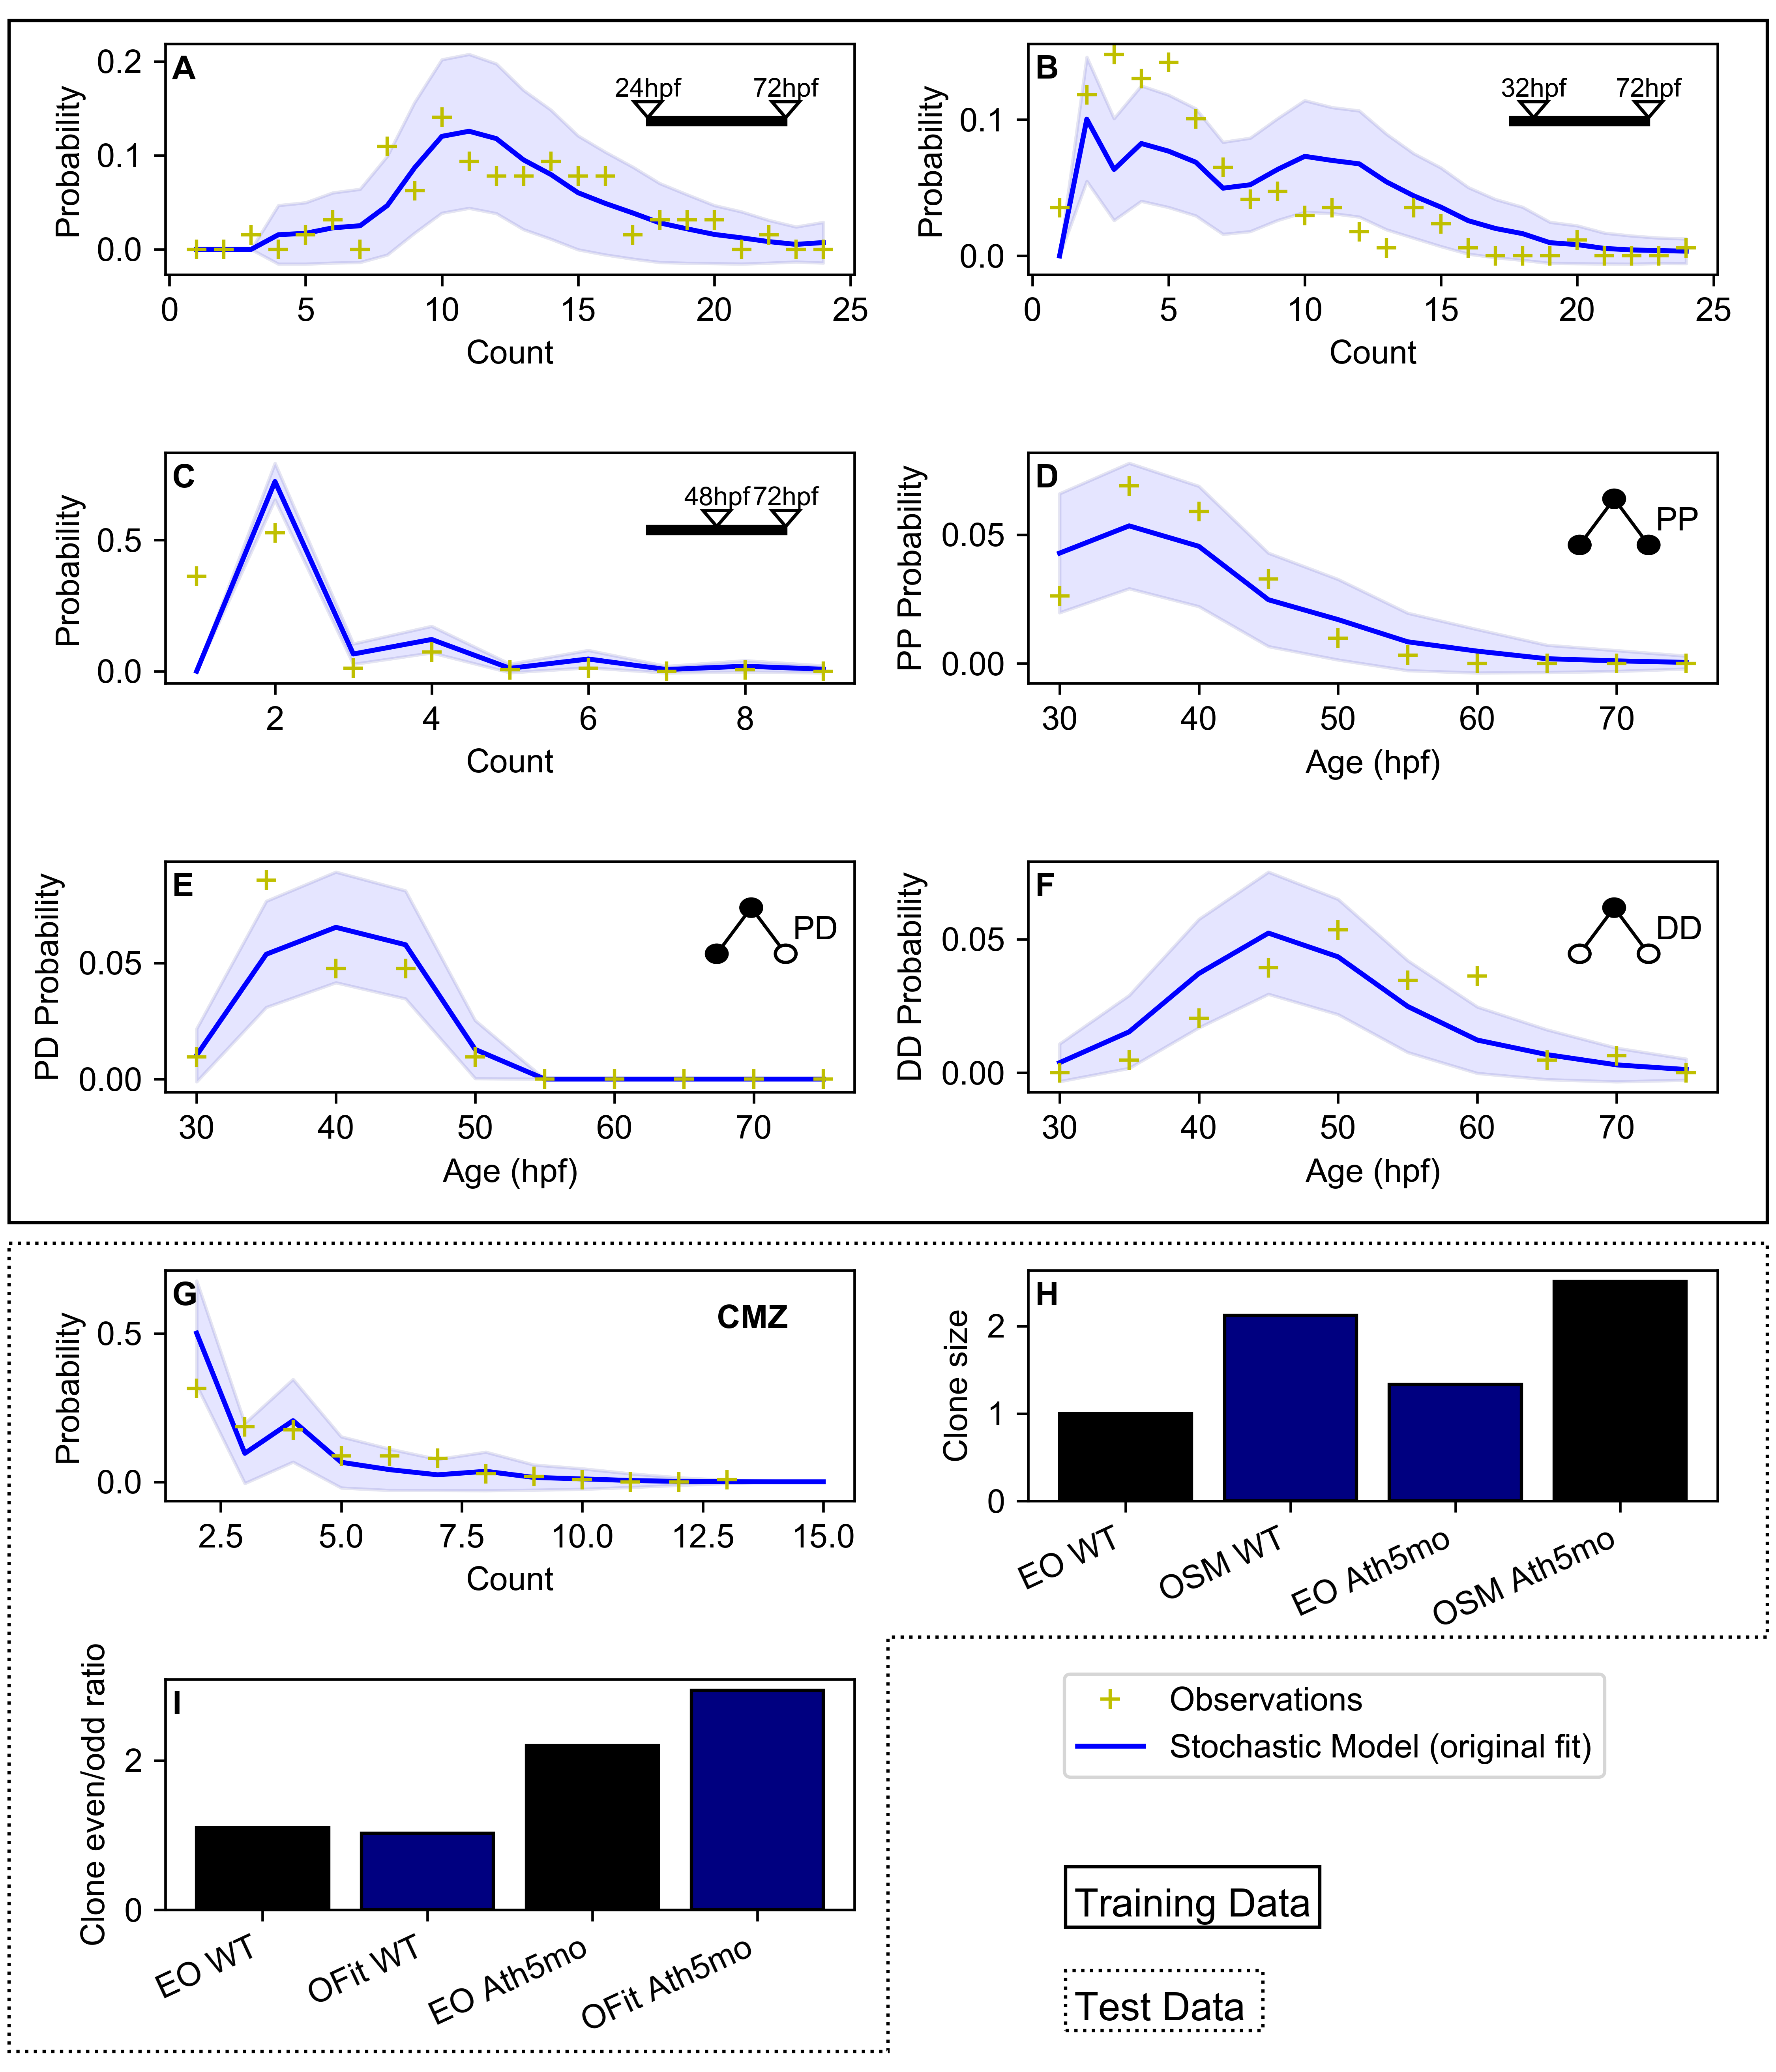
\includegraphics[width=1.\textwidth]{ssm/Fig_S1_o_fig.png}}
\paragraph{S1 Fig.}
\label{originalSupplement}
{\bf He SSM original parameterisation model output.} As Fig \ref{SDFig}; model output uses the parameterisation given in He et al.\cite{He2012}. Note significant deviation from observations in panel B, reflecting excess proliferative activity of modelled RPCs.
\end{figure}

\begin{figure}[p]
\makebox[\textwidth][c]{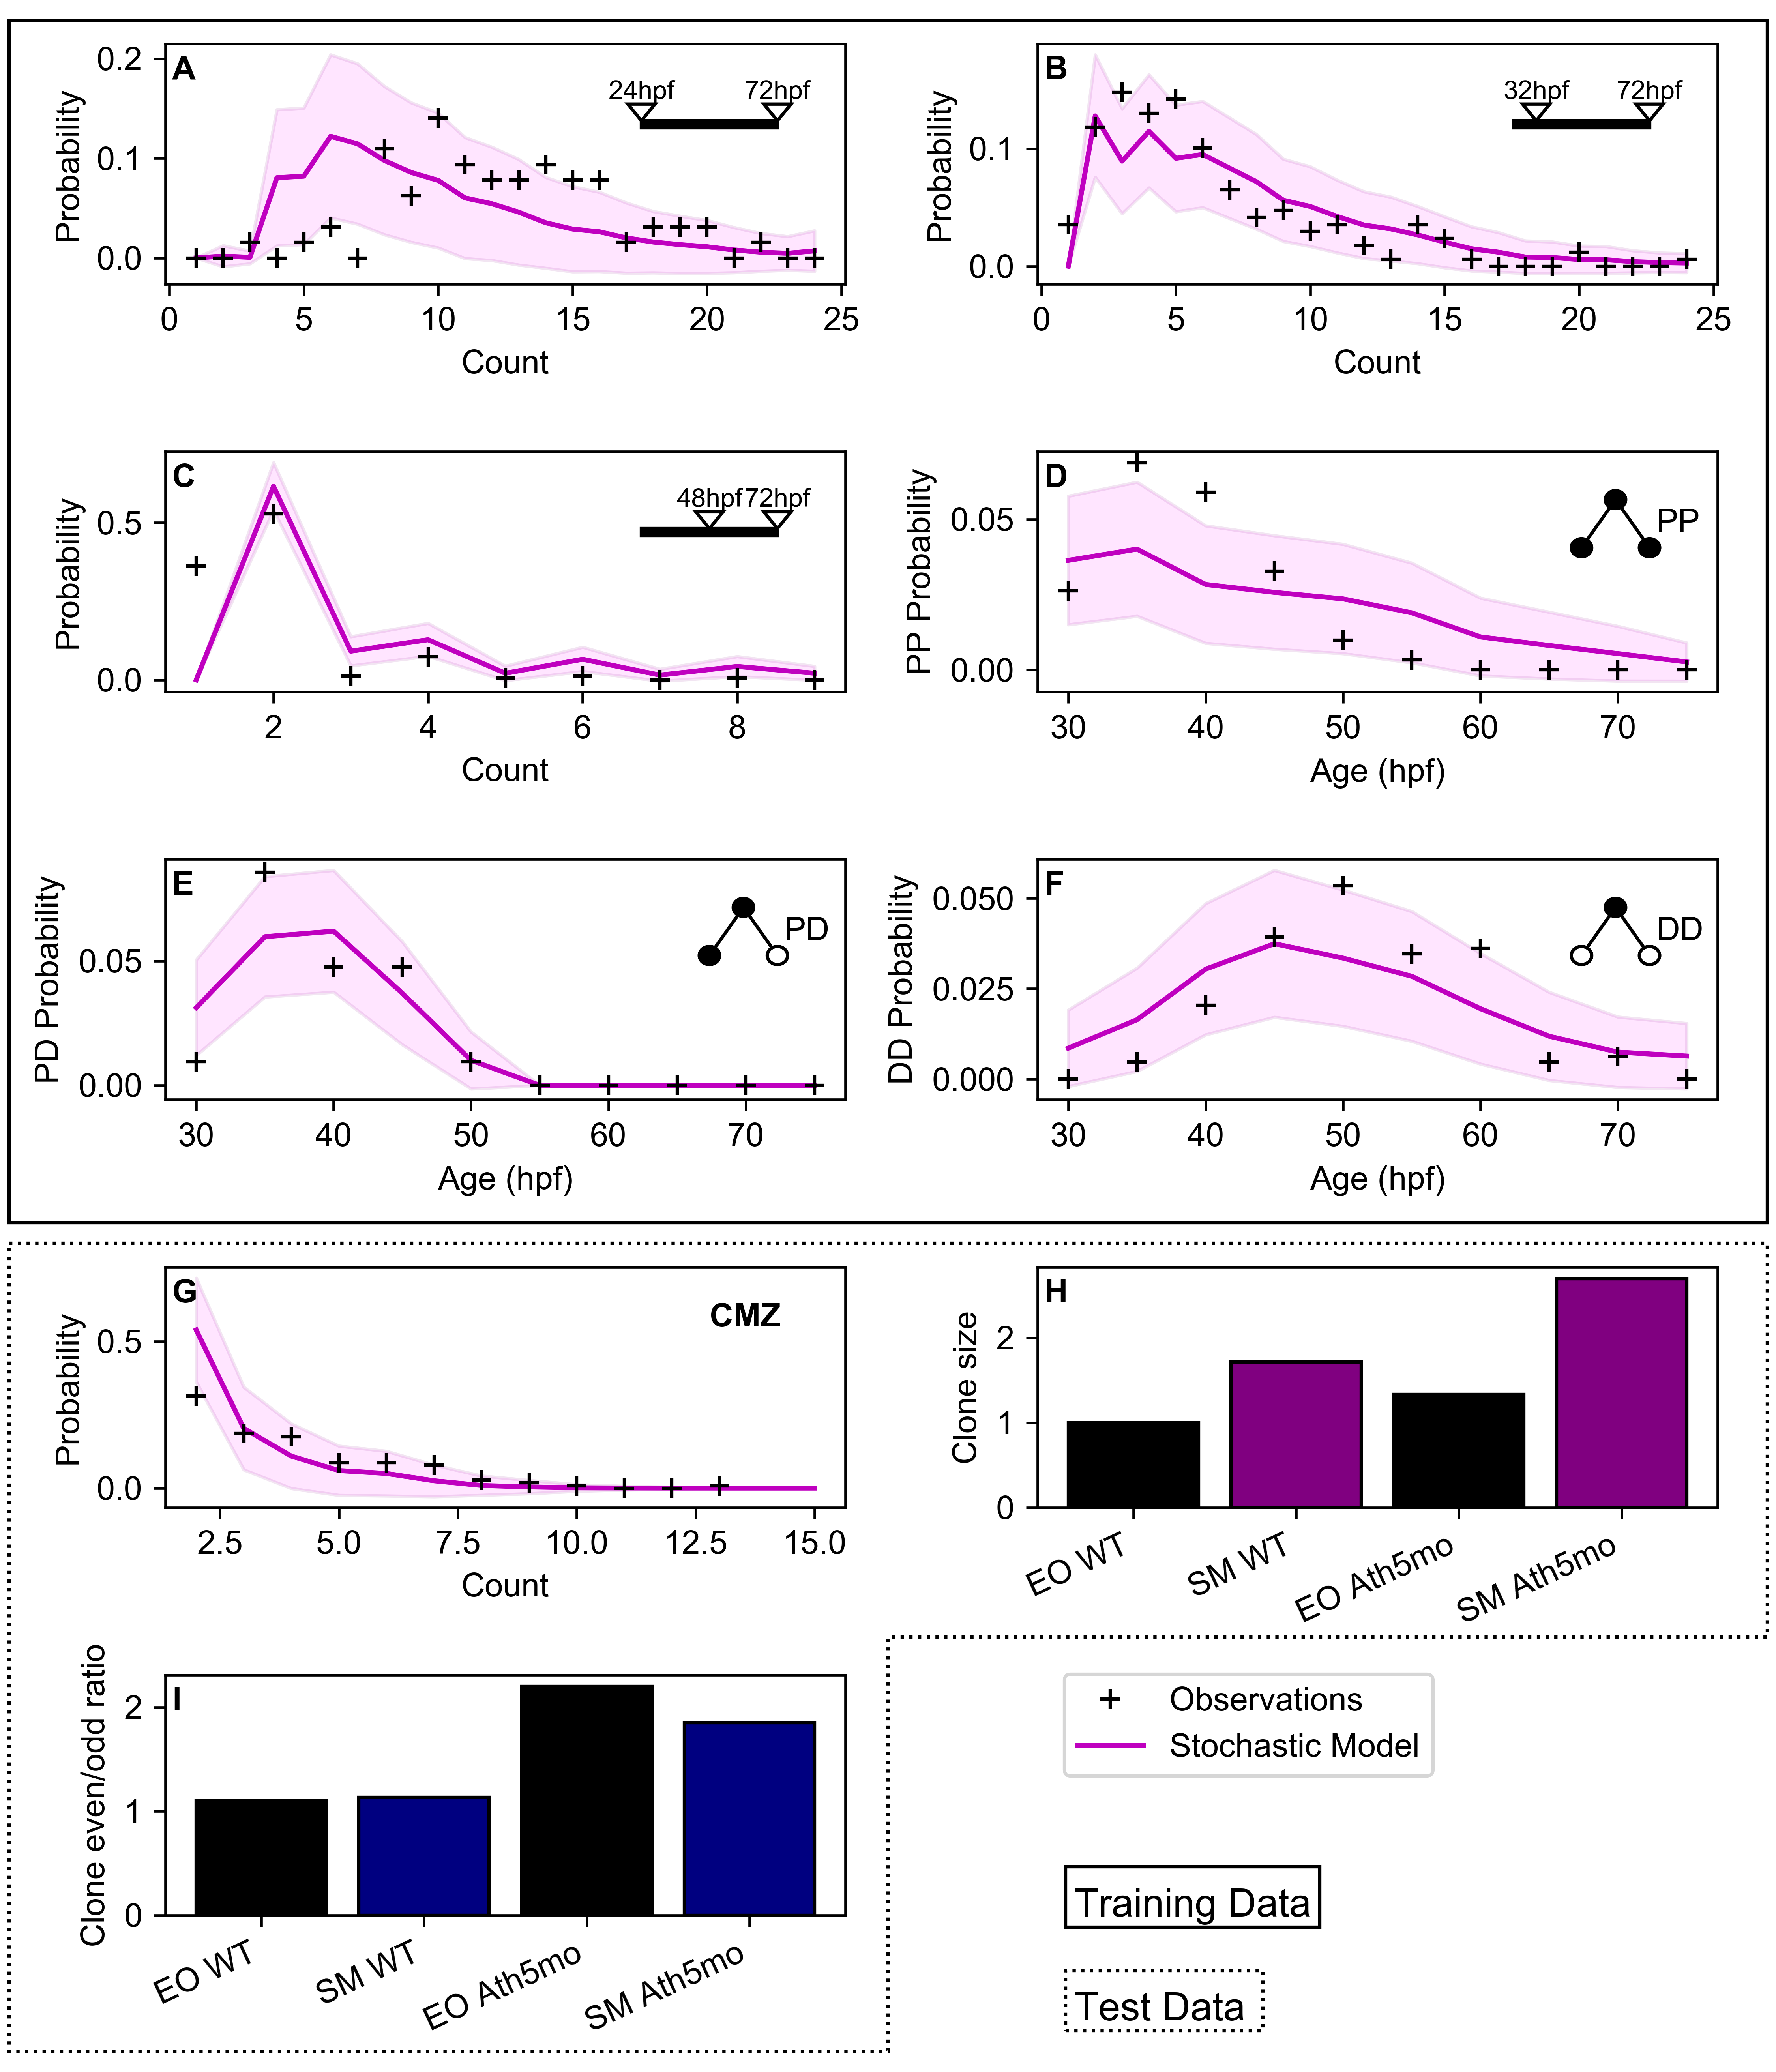
\includegraphics[width=1.\textwidth]{ssm/Fig_S2_s_fig.png}}
\paragraph{S2 Fig.}
\label{stochasticSupplement}
{\bf SPSA-optimised He SSM model output.} As Fig \ref{SDFig}; stochastic model output displayed alone.
\end{figure}

\begin{figure}[p]
\makebox[\textwidth][c]{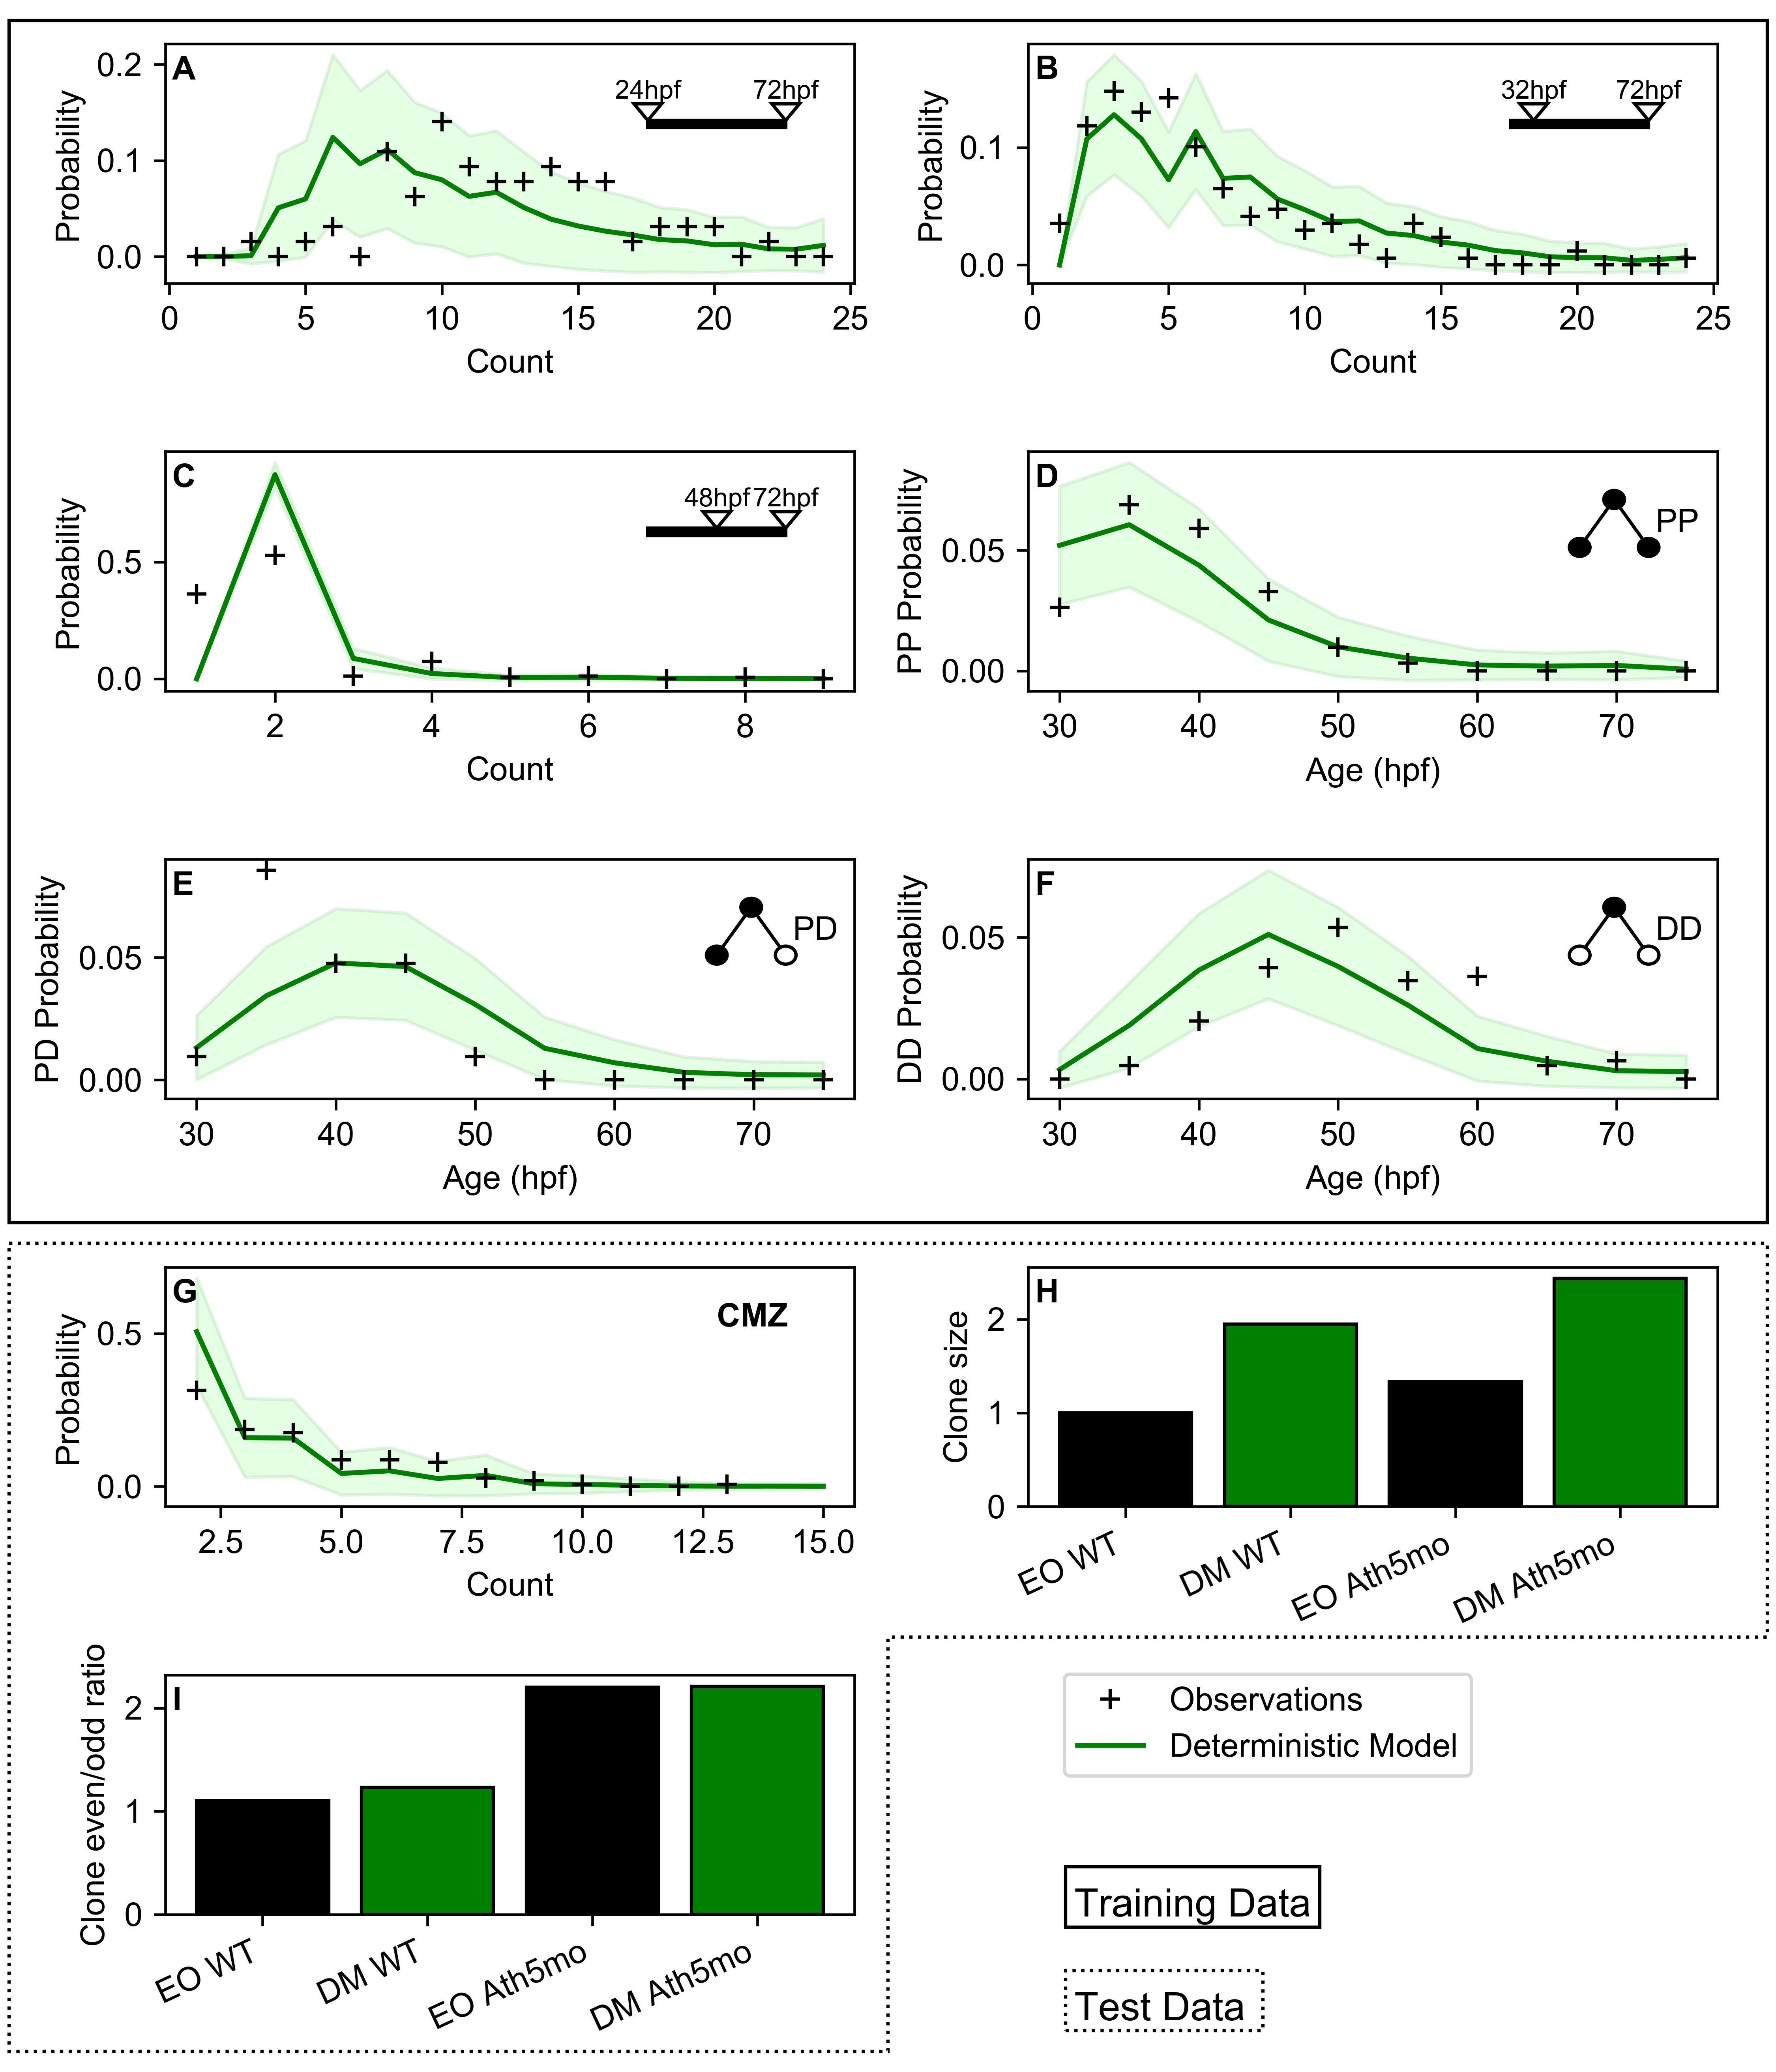
\includegraphics[width=1.\textwidth]{ssm/Fig_S3_d_fig.png}}
\paragraph{S3 Fig.}
\label{deterministicSupplement}
{\bf SPSA-optimised deterministic mitotic mode model output.} As Fig \ref{SDFig}; deterministic model output displayed by itself.
\end{figure}

\begin{figure}[h]
\makebox[\textwidth][c]{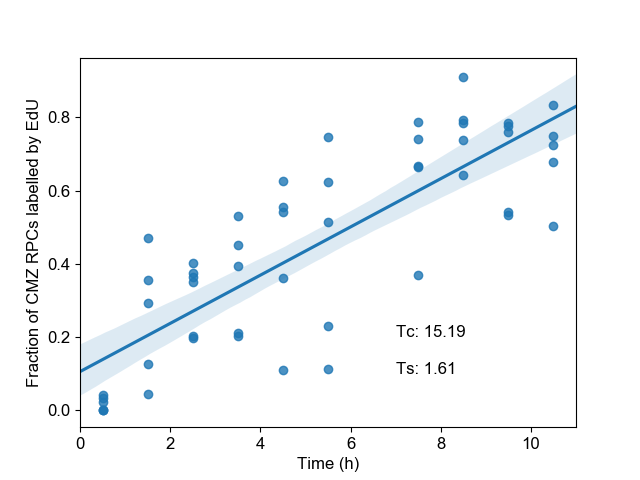
\includegraphics[width=1.\textwidth]{ssm/Fig_S4_cumulative_edu.png}}
\paragraph{S4 Fig.}
\label{cumulativeSupplement}
{\bf Cumulative EdU Labelling of 3dpf CMZ RPCs} Fraction of PCNA-labelled CMZ RPCs which bear EdU label over time, as determined by histochemical labelling of central coronal cryosections of 3dpf zebrafish retinas. Dots represent results from individual retinas. Line is the ordinary least squares fit $\pm$ 95\% CI. Cell cycle length (Tc) and S-phase length (Ts) are estimated from this fit following the method of Nowakowski et al.\cite{Nowakowski1989}
\end{figure}